% !TEX root =  main.tex

%Description of \m\mEdhoc and main changes from last verified version

\vnote{I find the macros for the protocol, method, and tool names distracting while reading through (the font changes too much, too often). The macro for EDHOC actually inserts a line break if you start a sentence with it, because of the \texttt{hbox} (I'm not sure why the hbox exists for what is a macro to be inserted in running text). I do need to start sentence with EDHOC many times though, so this is irritating. It is also the case that ProVerif needs to be written like so, and not capitalized entirely, so at least one of them is plain wrong! For now I've left in the macros, but I'd prefer that we fixed them to be regular capitalized text or, in the case of ProVerif, in camelcase as they should be.}

\subsection{Overview}
Constrained IoT systems often deal with a lot of valuable personal and business information that ought to be kept secure. Such systems need to be assured of end-to-end protection with source authentication and perfect forward secrecy. It is often desirable to protect such devices at the application layer -- for example, in cases where transport layer security is not sufficient [\mcneed], or where multiple underlying protocols need to be accounted for. One method for providing application layer security is provided by CBOR Object Signing and Encryption (COSE) [RFC8152: \mcfix].  

In order to derive shared key material with which to proceed, communicating parties can run an Elliptic Curve Diffie-Hellman key exchange protocol with ephemeral keys. Ephemeral Diffie-Hellman Over COSE (\mEdhoc) is a lightweight key exchange protocol for such situations, and is expected to provide perfect forward secrecy and identity protection. \mEdhoc supports authentication using pre-shared keys (PSK), raw public keys (RPK), and public key certificates. After successful completion of the \mEdhoc protocol, application keys and other application specific data can be derived using the \mEdhoc-Exporter interface. 

A main use case for \mEdhoc is to establish a security context for Object Security for Constrained RESTful Environments (\mOscore) [RFC8613: \mcfix]. \mOscore is a protocol which uses COSE for application-layer protection on top of the transport-layer Constrained Application Protocol (CoAP). \mEdhoc uses COSE for cryptography, CBOR for encoding, and CoAP for transport. By reusing existing libraries, the additional code footprint can be kept very low.

\mEdhoc is designed to work in highly constrained scenarios. This makes it especially suitable for network technologies which have low throughput, low power consumption, and small frame sizes. Examples include Cellular IoT, 6TiSCH, and LoRaWAN [\mcneed].

\subsection{Background, comparison with~\cite{DBLP:conf/secsr/BruniJPS18}}
The first version of \mEdhoc was proposed in March 2016 to a working group investigating lightweight authenticated key exchange protocols [\mcneed]. There has been a focus on formally verifying that the protocol satisfies the properties expected of it right from the beginning. 

The 2018 work~\cite{DBLP:conf/secsr/BruniJPS18} by Bruni et al performed a formal verification of version 08 [\url{https://tools.ietf.org/html/draft-selander-ace-cose-ecdhe-08} \mcfix] of \mEdhoc. The protocol and properties are modelled and verified in the \mProverif tool. This version of the protocol belongs to the \mSigmaI family of protocols, and has two modes -- one with asymmetric keys, and one with pre-shared symmetric keys (PSK). Bruni et al showed that this version satisfies the requisite properties of identity protection, (perfect forward) secrecy of data, and strong authentication, upon completion of the protocol.

\mEdhoc has undergone a lot of change since version 08, as will be described in the following sections, and the formal verification of the current version, therefore, is a worthwhile exercise.

%\subsection{Overarching goal of security context establishment}
\subsection{Methods and features of \textsc{EDHOC}}
\mEdhoc can established Diffie-Hellman key exchange in one of three different ways -- using digital signatures, static Diffie-Hellman keys, or pre-shared symmetric keys. We describe each of these methods in detail below. The communicating parties must agree on the method as part of the first message.

\subsubsection{\mSigSig method}
The \mSigma (SIGn-and-MAc) family of protocols [\mcneed] has many variants. The \mSigSig method of \mEdhoc is built on \mSigmaI, a variant of the \mSigma protocol which provides identity protection for the initiator, and  implements the \mSigmaI variant as Mac-then-Sign. The current \mSigSig method corresponds (with a few minor changes) to the asymmetric key mode of \mEdhoc v08. 

The communicating parties exchange ephemeral public keys, compute the shared secret, and derive symmetric application keys from this secret.

\subsubsection{\mPskPsk method}
In this method, the initiator and responder are assumed to have a pre-shared key which is secret to them, and can be retrieved by the responder using a public part of the first message (\mIDPSK). This method corresponds to the symmetric key method of \mEdhoc v08. 

In the first message, the initiator sends a message consisting of the method name, the initiator's ephemeral key (\mGx), their connection identifier (\mCi), the \mIDPSK identifier, and (optional) plaintext (\mADone). 

The second message, sent by the responder, is composed of \mCi, the responder's ephemeral key \mGy, their connection identifier \mCr, and an AEAD encryption [\mcneed] of the transaction hash of the first message (\mTHtwo) along with an optional plaintext \mADtwo. The key used for this (\mKtwo) is derived using the EDHOC key derivation function with \mTHtwo and the pseudorandom string \mPRKtwo as input, while the associated data for the AEAD encryption is constructed by concatenating a constant string, the hash function, and \mTHtwo. 

The initiator, upon receipt of this message, sends back \mCr, followed by an AEAD encryption of the transaction hash of the second message (\mTHthree) along with a plaintext \mADthree. As earlier, the key used is derived by supplying \mTHthree and \mPRKthree as input to the KDF, and the  associated data obtained by concatenating the constant string, hash function, and \mTHthree. An abstract description is shown in Figure~\ref{fig:edhocpsk}.

\vnote{Figure numbers don't square up, check class file guidelines!}

\begin{figure}\label{fig:edhocpsk}
\centering
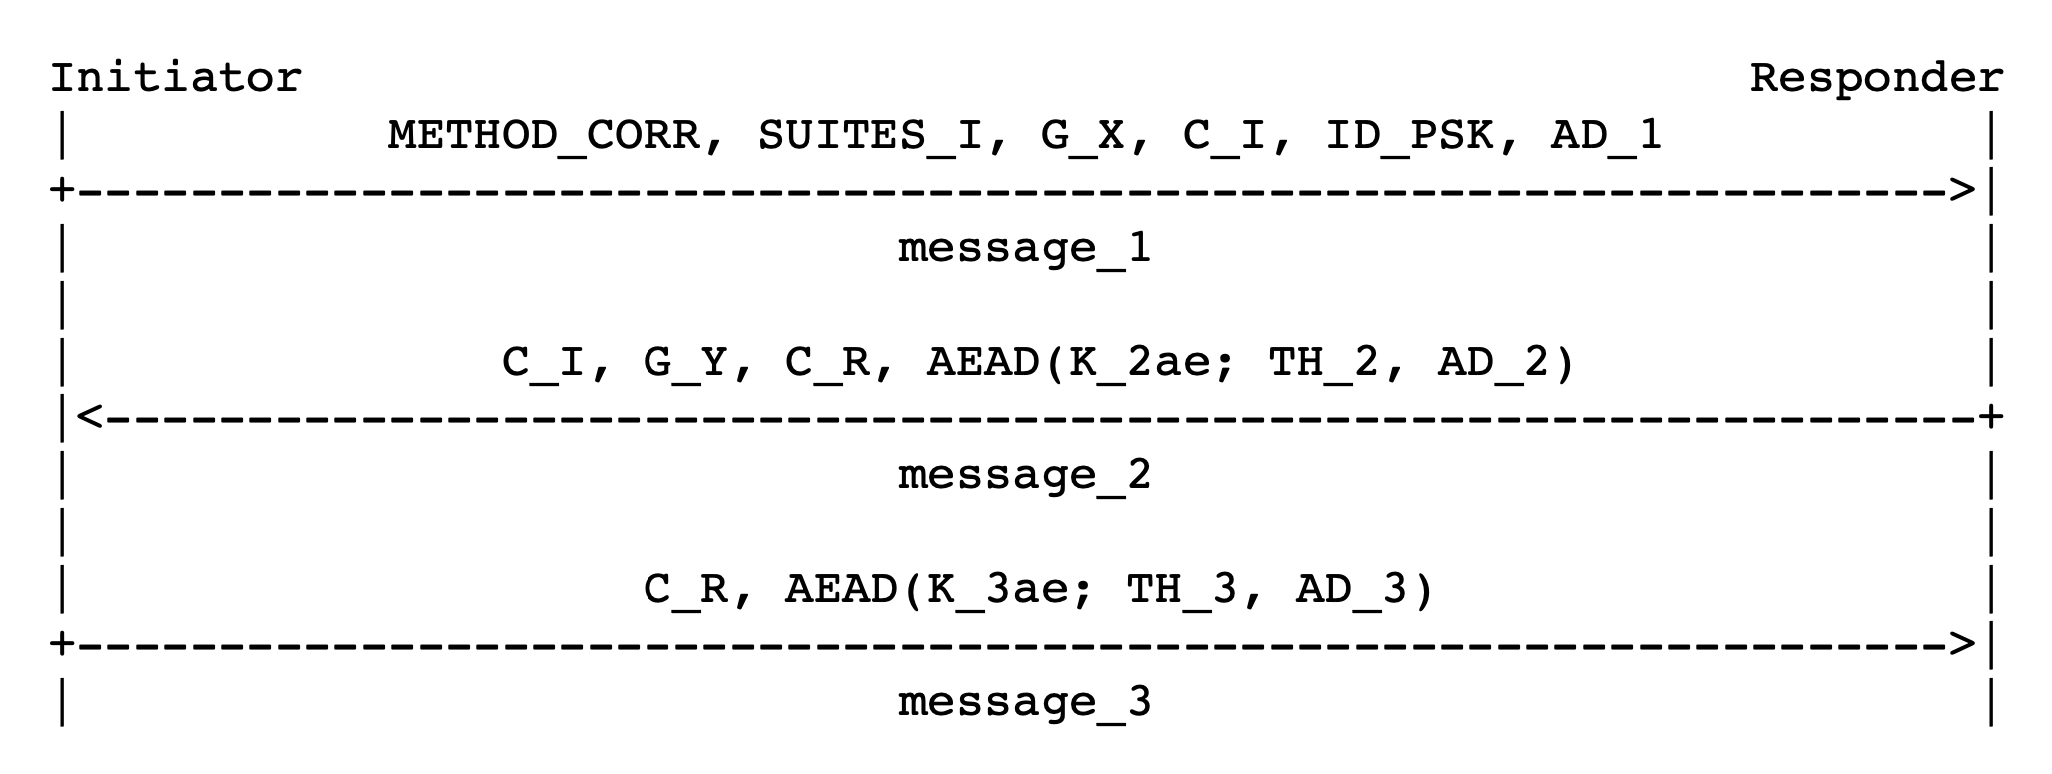
\includegraphics[scale=0.3]{Images/psk.png}
\caption{The PSK-PSK method of EDHOC}
\end{figure}

\subsubsection{\mStat-based methods}
\mEdhoc allows for three \mStat-based methods -- two where only one participant has a static Diffie-Hellman key (while the other uses signatures), and one where both do. This set of methods is not covered in v08 of \mEdhoc, which only has a single \mSigma asymmetric key method (corresponding to the \mSigSig method shown above). This allows one party to use a \mSigma style of authentication, while the other can use something along the lines of \mOptls.

\vnote{Need to talk about links to OPTLS and NOISE}



\subsection{Expected security properties}


%Discussion of KDF -- page 13 of EDHOC

%certain security applications may be integrated into EDHOC by transporting auxiliary data together with the messages. One example is the transport of third-party authorization information protected outside of EDHOC [I-D.selander-ace-ake-authz]. Another example is the embedding of a certificate enrolment request or a newly issued certificate. EDHOC allows opaque auxiliary data (AD) to be sent in the EDHOC messages. Unprotected Auxiliary Data (AD_1, AD_2) may be sent in message_1 and message_2, respectively. Protected Auxiliary Data (AD_3) may be sent in message_3. Since data carried in AD1 and AD2 may not be protected, and the content of AD3 is available to both the Initiator and the Responder, special considerations need to be made such that the availability of the data a) does not violate security and privacy requirements of the service which uses this data, and b) does not violate the security properties of EDHOC. 

